\documentclass[12pt]{beamer}
\usepackage{../Estilos/BeamerMAF}
\usetheme{Dresden}
\usecolortheme{seahorse}
%\useoutertheme{default}
\setbeamercovered{invisible}
% or whatever (possibly just delete it)
\setbeamertemplate{section in toc}[sections numbered]
\setbeamertemplate{subsection in toc}[subsections numbered]
\setbeamertemplate{subsection in toc}{\leavevmode\leftskip=3.2em\rlap{\hskip-2em\inserttocsectionnumber.\inserttocsubsectionnumber}\inserttocsubsection\par}
\setbeamercolor{section in toc}{fg=blue}
\setbeamercolor{subsection in toc}{fg=blue}
\setbeamercolor{frametitle}{fg=blue}
\setbeamertemplate{caption}[numbered]

\setbeamertemplate{footline}
\beamertemplatenavigationsymbolsempty
\setbeamertemplate{headline}{}

\makeatletter
\setbeamercolor{section in foot}{bg=gray!30, fg=black!90!orange}
\setbeamercolor{subsection in foot}{bg=blue!30!yellow, fg=red}
\setbeamertemplate{footline}
{
  \leavevmode%
  \hbox{%
  \begin{beamercolorbox}[wd=.333333\paperwidth,ht=2.25ex,dp=1ex,center]{section in foot}%
    \usebeamerfont{section in foot} \insertsection
  \end{beamercolorbox}}%
  \begin{beamercolorbox}[wd=.333333\paperwidth,ht=2.25ex,dp=1ex,center]{subsection in foot}%
    \usebeamerfont{subsection in foot}  \insertsubsection
  \end{beamercolorbox}%
  \begin{beamercolorbox}[wd=.333333\paperwidth,ht=2.25ex,dp=1ex,right]{date in head/foot}%
    \usebeamerfont{date in head/foot} \insertshortdate{} \hspace*{2em}
    \insertframenumber{} / \inserttotalframenumber \hspace*{2ex} 
  \end{beamercolorbox}}%
  \vskip0pt%
\makeatother 

\makeatletter
\patchcmd{\beamer@sectionintoc}{\vskip1.5em}{\vskip0.8em}{}{}
\makeatother


\date{10 de noviembre de 2021}

\title{\large{Álgebra de kets y bras}}
\author{M. en C. Gustavo Contreras Mayén}

\begin{document}
\maketitle
\fontsize{14}{14}\selectfont
\spanishdecimal{.}

\section*{Contenido}
\frame{\tableofcontents[currentsection, hideallsubsections]}


%Ref. Ghatak (2004) Quantum Mechanics. Chap. 11
\section{La notación de bras y kets}
\frame{\tableofcontents[currentsection, hideothersubsections]}
\subsection{Definiciones}

\begin{frame}
\frametitle{Los bras y los kets}
En esta sesión presentaremos de manera general el álgebra bra y ket de Dirac en la que los estados de un sistema dinámico se denotarán mediante ciertos vectores (que, siguiendo a Dirac, se denominarán vectores bra y ket)
\end{frame}
\begin{frame}
\frametitle{Los bras y los kets}
Los operadores que representan variables dinámicas (como coordenadas de posición, componentes del momento y momento angular) mediante matrices.
\end{frame}
\begin{frame}
\frametitle{El ket}
El estado de un sistema se puede representar mediante un cierto tipo de vector, \pause que llamamos vector \emph{ket} y representamos con el símbolo $\ket{ \quad }$.
\\
\bigskip
\pause
Para distinguir los vectores ket correspondientes a diferentes estados, insertamos una etiqueta; así, el vector ket (o simplemente el ket) correspondiente al estado $A$ se describe con el símbolo $\ket{A}$.
\end{frame}
\begin{frame}
\frametitle{El espacio vectorial de los kets}
Las kets forman un espacio vectorial lineal, lo que implica que si tenemos dos estados descritos por las kets $\ket{A}$ e $\ket{B}$, entonces la combinación lineal:
\pause
\begin{align*}
c_{1} \, \ket{A} + c_{2} \, \ket{B}
\end{align*}
\pause
es un vector en el mismo espacio vectorial, en esta ecuación, $c_{1}$ y $c_{2}$ son dos números complejos arbitrarios.
\end{frame}
\begin{frame}
\frametitle{Lo que pensaba Dirac}
Para citar a Dirac:
\begin{quote}
... cada estado de un sistema dinámico en un momento particular corresponde a un vector ket; siendo la correspondencia tal que si un estado resulta de la superposición de ciertos otros estados, su vector ket correspondiente es expresable linealmente en términos de los vectores ket correspondientes de los otros estados, y viceversa.
\end{quote}
\end{frame}
\begin{frame}
\frametitle{Correspondencia de los kets}
Además, el ket $\ket{A}$ y $c \, \ket{A}$ (donde $c$ es un número complejo arbitrario distinto de cero) corresponden al mismo estado.
\\
\bigskip
\pause
En otras palabras, el estado del sistema está definido por la \enquote{dirección} de los vectores.
\end{frame}
\begin{frame}
\frametitle{Principio de superposición}
A este respecto, el principio de superposición en las teorías clásica y cuántica difieren.
\\
\bigskip
\pause
Por ejemplo, la superposición de una cuerda oscilando sobre sí misma da, en la física clásica, un modo con el doble de amplitud y cuatro veces la energía del estado inicial de vibración.
\\
\bigskip
\pause
Por el contrario, en la mecánica cuántica, \emph{la superposición de un estado sobre sí mismo da el mismo estado}.
\end{frame}
\begin{frame}
\frametitle{Espacio dual}
Ahora, con cada espacio vectorial se puede asociar un espacio vectorial dual de modo que se pueda formar un producto escalar de los dos vectores, uno de cada espacio.
\\
\bigskip
\pause
Los vectores del espacio dual al de los vectores ket se denominarán vectores bra o simplemente \enquote{bras} y se denotarán por $\bra{ \quad }$.
\end{frame}
\begin{frame}
\frametitle{El producto escalar}
El producto escalar del ket $\ket{A}$ y el bra $\bra{B}$ se denota por $\braket{B}{A}$ y es un número complejo.
\\
\bigskip
\pause
La lógica es muy similar a la que se tiene en la teoría de matrices donde a cada vector columna se le puede asociar un vector fila y el producto escalar de los dos devuelve un número.
\end{frame}

\subsection{Propiedades de los bras y los kets}

\begin{frame}
\frametitle{Bra nulo}
Se dice que un bra es un bra nulo si el producto escalar se anula para cualquier ket, es decir:
\pause
\begin{align*}
\bra{B} = 0 \hspace{0.3cm} \mbox{si} \hspace{0.4cm} \braket{B}{A} = 0 \hspace{0.3cm} \mbox{para cualquier} \hspace{0.3cm} \ket{A}
\end{align*}
\end{frame}
\begin{frame}
\frametitle{Bras iguales}
Se dice que dos bras son iguales si su producto escalar con un ket arbitrario son iguales, por lo tanto:
\pause
\begin{align*}
\bra{B_{1}} = \bra{B_{2}} \hspace{0.3cm} &\mbox{si} \hspace{0.3cm} \braket{B_{1}}{A} = \braket{B_{2}}{A} \\[0.5em]
&\mbox{para cualquier} \hspace{0.3cm} \ket{A}
\end{align*}
\end{frame}
\begin{frame}
\frametitle{Correspondencia entre bras y kets}
Se asume además que:
\pause
\setbeamercolor{item projected}{bg=blue!70!black,fg=yellow}
\setbeamertemplate{enumerate items}[circle]
\begin{enumerate}[<+->]
\item Existe una correspondencia uno a uno entre kets y bras en el sentido de que un estado de un sistema dinámico representado por $\ket{A}$ está igualmente bien representado por el bra correspondiente $\bra{A}$. Además, si:
\pause
\begin{align*}
\ket{P} = \ket{A} + \ket{B} \hspace{0.3cm} \mbox{entonces} \hspace{0.3cm} \bra{P} = \bra{A} + \bra{B}
\end{align*}
\seti
\end{enumerate}
\end{frame}
\begin{frame}
\frametitle{Correspondencia entre bras y kets}
Y si:
\pause
\begin{align*}
\ket{R} = c \, \ket{A} \hspace{0.3cm} \mbox{entonces} \hspace{0.3cm} \bra{R} = c^{*} \, \bra{A}
\end{align*}
donde $c$ es un número complejo y $c^{*}$ es su conjugado complejo.
\end{frame}
\begin{frame}
\frametitle{Correspondencia entre bras y kets}
\setbeamercolor{item projected}{bg=blue!70!black,fg=yellow}
\setbeamertemplate{enumerate items}[circle]
\begin{enumerate}[<+->]    
\conti
\item \begin{align*}
\braket{A}{B} = \braket{B}{A}^{*}
\end{align*}
donde el ${}^{*}$ representa el complejo conjugado de la cantidad. 
\end{enumerate}
\pause
Haciendo que: $\ket{B} = \ket{A}$, se tiene:
\pause
\begin{align*}
\braket{A}{A} = \braket{A}{A}^{*}
\end{align*}
lo que implica que el producto escalar $\braket{A}{A}$ es un número real.
\end{frame}
\begin{frame}
\frametitle{Valor del producto escalar}
Es posible afirmar que:
\pause
\begin{align*}
\braket{A}{A} \geq 0
\end{align*}
\pause
el signo de igualdad se presenta solo cuando $\ket{A} = 0$, es decir, cuando $\ket{A}$ es el ket nulo.
\end{frame}
\begin{frame}
\frametitle{Ortogonalidad en los kets}
Si $\braket{A}{B} = 0$ entonces lo kets $\ket{A}$ y $\ket{B}$ se dice que son ortogonales entre ellos.
\end{frame}
\begin{frame}
\frametitle{Ket normalizado}
Si $\braket{A}{A} = 1$, entonces se dice que el ket $\ket{A}$ está normalizado.
\\
\bigskip
\pause
Dado que los kets $\ket{A}$ y $c \, \ket{A}$ corresponden al mismo estado, siempre podemos asociar kets normalizados a cada estado. \pause Puede verse fácilmente que un ket normalizado se define solo dentro de un factor de fase arbitrario $e^{i \gamma}$ (donde $\gamma$ es un número real).
\end{frame}
\begin{frame}
\frametitle{Relación con la mecánica cuántica}
Podemos mencionar la relación entre las funciones de onda de Schrödinger con los bra y kets.
\\
\bigskip
\pause
Si $\ket{\psi}$ e $\ket{\phi}$ representan las kets correspondientes a los estados descritos por las funciones de onda $\psi(\vb{r})$ y $\phi(\vb{r})$ respectivamente.
\end{frame}
\begin{frame}
\frametitle{Producto escalar}
Se define el producto escalar:
\pause
\begin{align*}
\braket{\phi}{\psi} = \scaleint{6ex} \, \phi^{*} (\vb{r}) \, \psi (\vb{r}) \dd{\tau} = \braket{\psi}{\phi}^{*}
\end{align*}
donde la integración se realiza en todo el espacio. Esta integral se refiere como el producto escalar de dos funciones.
\end{frame}

\section{Operadores lineales}
\frame{\tableofcontents[currentsection, hideothersubsections]}
\subsection{Operadores, bras y kets}

\begin{frame}
\frametitle{Operadores y kets}
Un operador $\alpha$ convierte un ket $\ket{A}$ en otro ket $\ket{B}$:
\pause
\begin{align*}
\ket{B} = \alpha \, \ket{A}
\end{align*}
\end{frame}
\begin{frame}
\frametitle{Operador lineal}
Un operador se dice que es lineal si satisface la siguiente ecuación:
\pause
\begin{align*}
\alpha \, \big( c_{1} \ket{A_{1}} {+} c_{2} \ket{A_{2}} {+} \cdots  \big) = c_{1} \alpha \ket{A_{1}} {+} c_{2} \alpha \ket{A_{2}} + \cdots
\end{align*}
donde $c_{1}, c_{2}, \ldots$ son números complejos arbitrarios. De ahora en adelante, consideraremos solo operadores lineales.
\end{frame}
\begin{frame}
\frametitle{Operador nulo}
Se dice que un operador $\alpha$ es un \emph{operador nulo} si:
\pause
\begin{align*}
\alpha \, \ket{A} = 0 \hspace{0.4cm} \mbox{para cualquier} \hspace{0.2cm} \ket{A}
\end{align*}
\pause
Por tanto, una condición necesaria y suficiente para que un operador sea un operador nulo es:
\pause
\begin{align*}
\mel{A}{\alpha}{A} = 0 \hspace{0.4cm} \mbox{para cualquier} \hspace{0.2cm} \ket{A}
\end{align*}
\end{frame}
\begin{frame}
\frametitle{Operador unitario}
Se dice que un operador es \emph{unitario} si:
\pause
\begin{align*}
\alpha \, \ket{A} = \ket{A} \hspace{0.4cm} \mbox{para cualquier} \hspace{0.2cm} \ket{A}
\end{align*}
\pause
Puede verse fácilmente que un número puede considerarse un operador lineal.
\end{frame}
\begin{frame}
\frametitle{Dos operadores iguales}
Se dice que dos operadores $\alpha$ y $\beta$ son iguales si y solo si:
\pause
\begin{align*}
\mel{A}{\alpha}{A} = \mel{A}{\beta}{A} \hspace{0.4cm} \mbox{para cualquier} \hspace{0.2cm} \ket{A}
\end{align*}
\end{frame}
\begin{frame}
\frametitle{Suma/Diferencia en operadores}
La suma (o diferencia) de dos operadores $\alpha$ y $\beta$ se define mediante la ecuación:
\pause
\begin{align*}
\big( \alpha \pm \beta \big) \, \ket{A} = \alpha \, \ket{A} \pm \beta \, \ket{A}
\end{align*}
\end{frame}
\begin{frame}
\frametitle{Propiedades de los operadores}
Con lo anterior, podemos presentar:
\\
\pause
Ley asociativa:
\pause
\begin{align*}
\alpha + \big( \beta + \gamma \big) = \big( \alpha + \beta \big) + \gamma = \alpha + \beta + \gamma
\end{align*}
\end{frame}
\begin{frame}
\frametitle{Propiedades de los operadores}
También:
\pause
\begin{align*}
\big( c_{1} \, \alpha \big) \, \ket{A} = c_{1} \, \big( \alpha \, \ket{A} \big)
\end{align*}
donde $c_{1}$ es una constante compleja arbitraria.
\end{frame}
\begin{frame}
\frametitle{Producto de dos operadores}
El producto de dos operadores $\alpha$ y $\beta$ está
definido a través de la ecuación:
\pause
\begin{align*}
\big( \beta \, \alpha \big) \, \ket{A} = \beta \, \big( \alpha \, \ket{A} \big) = \beta \, \ket{B}
\end{align*}
donde $\ket{B} = \alpha \, \ket{A}$.
\\
\bigskip
\pause
En general:
\begin{align*}
\beta \, \alpha \neq \alpha \, \beta
\end{align*}
\end{frame}
\begin{frame}
\frametitle{El conmutador}
El \emph{conmutador} de dos operadores está definido por: 
\pause
\begin{align*}
\big[ \alpha, \beta \big] = \alpha \, \beta - \beta \, \alpha = - \big[ \beta, \alpha \big]
\end{align*}
\end{frame}
\begin{frame}
\frametitle{Operadores y bras}
Hasta ahora hemos asumido que un operador lineal actúa sobre kets; \pause también podemos hacer que un operador lineal $\alpha$ opere los bras.
\\
\bigskip
\pause
La regla es que el bra se tiene que poner a la izquierda del operador como $\bra{P}  \, \alpha$.
\end{frame}
\begin{frame}
\frametitle{Operadores y bras}
La operación se define a través de la ecuación:
\pause
\begin{eqnarray*}
\begin{aligned}
\left\{ \bra{P} \, \alpha \right\} \, \ket{A} &= \bra{P} \, \left\{ \alpha \, \ket{A} \right\} \hspace{0.4cm} \mbox{para cualquier} \hspace{0.2cm} \ket{A} \\[0.5em] \pause
&= \braket{P}{B}
\end{aligned}
\end{eqnarray*}
donde:
\begin{align*}
\ket{B} = \alpha \, \ket{A}
\end{align*}
\end{frame}
\begin{frame}
\frametitle{Nota importante}
La combinación $\alpha \, \bra{B}$ no tiene sentido.
\\
\bigskip
\pause
De hecho, debido a la ley asociativa no se necesita poner corchetes y simplemente escribir:
\pause
\begin{align*}
\mel{P}{\alpha \, \beta \, \gamma}{A}
\end{align*}
\end{frame}
\begin{frame}
\frametitle{}
Es interesante notar que la combinación $\ket{B} \, \bra{A}$ puede considerarse como un operador porque:
\pause
\begin{eqnarray*}
\begin{aligned}
\left\{ \ket{B} \, \bra{A} \right\} \, \ket{P} &= \ket{B} \, \left\{ \braket{A}{P} \right\} \\[0.5em] \pause
&= c \, \ket{B}
\end{aligned}
\end{eqnarray*}
\pause
porque $\braket{A}{P} \, (= c)$ es solo un número complejo.
\end{frame}
\begin{frame}
\frametitle{Adjunto de un operador}
% \emph{Adjunto de un operador}.
El adjunto del operador $\alpha$ se denota por $\alpha^{\dagger}$ y se define mediante la ecuación:
\pause
\begin{align*}
\mel{A}{\alpha^{\dagger}}{B} = \mel{B}{\alpha}{A}^{*}
\end{align*}
donde $\mel{B}{\alpha}{A}^{*}$ es el conjugado complejo del número $\mel{A}{\alpha^{\dagger}}{B}$.
\end{frame}
\begin{frame}
\frametitle{Adjunto de un operador}
Ahora:
\pause
\begin{eqnarray}
\begin{aligned}[b]
\mel{A}{\big( \alpha^{\dagger} \big)^{\dagger}}{B} &= \mel{A}{\beta^{\dagger}}{B} \hspace{1cm} \big( \beta^{\dagger} \equiv \alpha \big) \\[0.5em] \pause
&= \mel{B}{\beta}{A}^{*} = \mel{B}{\alpha^{\dagger}}{A}^{*} = \\[0.5em] \pause
&= \big( \mel{A}{\alpha}{B}^{*} \big)^{*} = \mel{A}{\alpha}{B}
\end{aligned}
\label{eq:ecuacion_22}
\end{eqnarray}
porque el conjugado complejo del conjugado complejo de un número es el número original en sí mismo.
\end{frame}
\begin{frame}
\frametitle{Adjunto de un operador}
Dado que la ec. (\ref{eq:ecuacion_22}) se cumple para $\ket{A}$ y $\ket{B}$ arbitrarios, se tiene:
\pause
\begin{align*}
\big( \alpha^{\dagger} \big)^{\dagger} = \alpha
\end{align*}
\end{frame}
\begin{frame}
\frametitle{Propiedades del adjunto de un operador}
Es decir, el adjunto del adjunto de un operador lineal es el operador original en sí. \pause Además, el adjunto del producto de los dos operadores $\alpha$ y $\beta$ es el producto del adjunto de los dos operadores en orden inverso, esto es:
\pause
\begin{align*}
\alpha^{\dagger} \, \beta^{\dagger} = \beta^{\dagger} \, \alpha^{\dagger}
\end{align*}
\end{frame}
\begin{frame}
\frametitle{Operador autoadjunto}
Se dice que un operador es autoadjunto si:
\pause
\begin{align*}
\alpha^{\dagger} = \alpha
\end{align*}
Un operador autoadjunto es llamado \emph{operador real} o también \emph{operador Hermitiano}.
\end{frame}

\section{La ecuación de valores propios}
\frame{\tableofcontents[currentsection, hideothersubsections]}
\subsection{Ecuación con bras y kets}

\begin{frame}
\frametitle{La ecuación con valores propios}
Para el operador lineal $\alpha$, considera la ecuación:
\pause
\begin{align*}
\alpha \, \ket{A_{n}} = a_{n} \, \ket{A_{n}}
\end{align*}
donde $a_{n}$ es un número complejo arbitrario.
\\
\bigskip
\pause
La ecuación anterior representa una ecuación de valores propios.
\end{frame}
\begin{frame}
\frametitle{El ket como un conjunto propio}
Se dice que $\ket{A_{n}}$ es un \emph{conjunto propio} del operador $\alpha$, siendo $a_{n}$ todos los valores propios correspondientes.
\\
\bigskip
\pause
Puede verse fácilmente que $c \, \ket{A_{n}}$ (donde $c$ es un número complejo arbitrario) también es un \emph{eigenket} que pertenece al mismo valor propio $a_{n}$.
\end{frame}
\begin{frame}
\frametitle{El ket linealmente independiente}
Un ket $\ket{P}$ se dice que es linealmente independiente de los kets $\ket{A_{1}}, \ket{A_{2}}, \ldots, \ket{A_{N}}$ si podemos escribir:
\begin{align*}
\ket{P} = \nsum_{n=1}^{N} c_{n} \, \ket{A_{n}}
\end{align*}
\end{frame}
\begin{frame}
\frametitle{El ket como un conjunto propio}
Ahora, si hay más de un ket (y éstos no son linealmente dependientes entre sí) pertenecientes al mismo valor propio, es decir, si:
\pause
\\
\emph{Degeneración}.
\begin{eqnarray}
\alpha \, \ket{A_{1}} &= a_{1} \, \ket{A_{1}} \label{eq:ecuacion_31} \\[0.5em] \pause
\alpha \, \ket{A_{2}} &= a_{1} \, \ket{A_{2}} \label{eq:ecuacion_32}
\end{eqnarray}
entonces se dice que el estado es un \emph{estado degenerado}.
\end{frame}
\begin{frame}
\frametitle{Estados degenerados}
Si hay $g$ kets linealmente independientes que pertenecen al mismo valor propio, \pause entonces se dice que el estado está $g$-veces degenerado.
\\
\bigskip
\pause
En aras de la simplicidad, consideremos un estado degenerado doble descrito por las ecs. (\ref{eq:ecuacion_31}) y (\ref{eq:ecuacion_32}).
\end{frame}
\begin{frame}
\frametitle{Estados degenerados}
Si multiplicamos la ec. (\ref{eq:ecuacion_31}) por $c_{1}$ y la ec. (\ref{eq:ecuacion_32}) por $c_{2}$ y sumamos, obtendríamos:
\pause
\begin{align*}
\alpha \, \ket{P} = a_{1} \, \ket{P}
\end{align*}
donde:
\pause
\begin{align*}
\ket{P} = c_{1} \, \ket{A_{1}} + c_{2} \, \ket{A_{2}}
\end{align*}
lo que implica que la combinación lineal $c_{1} \, \ket{A_{1}} + c_{2} \, \ket{A_{2}}$ es también un eigenket que pertenece al mismo valor propio. %De manera similar, se puede discutir por un estado degenerado $g$-veces.
\end{frame}

\section{Ortogonalidad de las funciones propias}
\frame{\tableofcontents[currentsection, hideothersubsections]}
\subsection{Kets ortogonales}

\begin{frame}
\frametitle{Valores propios reales}
Cuando el valor $\alpha$ es real, se puede demostrar fácilmente que todos los valores propios son reales \pause y para dos valores propios diferentes (es decir, $a_{n} \neq a_{m}$) \pause las funciones propias correspondientes son necesariamente ortogonales, es decir:
\pause
\begin{align*}
\ip{A_n}{A_{m}} = 0 \hspace{1cm} a_{n} \neq a_{m}
\end{align*}
\end{frame}
\begin{frame}
\frametitle{Kets normalizados}
Además, siempre se pueden normalizar las kets y elegir una combinación lineal apropiada para los kets que pertenecen a un estado degenerado tal que:
\begin{align*}
\ip{A_{n}}{A_{m}} = \delta_{n m}
\end{align*}
\end{frame}

% La demostración es muy simple. Multiplicamos por la izquierda la ec. (\ref{eq:ecuacion_30}) por $\bra{A_{n}}$, para obtener:
% \begin{align*}
% \mel{A_{n}}{\alpha}{A_{n}} = a_{n} \, \ip{A_{n}}{A_{n}}
% \end{align*}
% Ahora $\ip{A_{n}}{A_{n}}$ es siempre real y no un ket nulo (de lo contrario, la ec. (\ref{eq:ecuacion_30}) no tiene
% sentido). Además, dado que $\alpha$ es real:
% \begin{align*}
% \mel{A_{n}}{\alpha}{A_{n}} = \mel{A_{n}}{\alpha^{\dagger}}{A_{n}} = \mel{A_{n}}{\alpha}{A_{n}}^{*}
% \end{align*}
% lo que implica que $\mel{A_{n}}{\alpha}{A_{n}}$ también es real y, por tanto, $a_{n}$ debe ser real. Además, para probar la ec. (\ref{eq:ecuacion_33}) consideramos:
% \begin{align}
% \alpha \, \ket{A_{1}} &= a_{1} \, \ket{A_{1}} \label{eq:ecuacion_35} \\
% \alpha \, \ket{A_{2}} &= a_{2} \, \ket{A_{2}} \label{eq:ecuacion_36}
% \end{align}
% Si hacemos que $\ket{P} = \alpha \, \ket{A_{2}}$, entonces:
% \begin{align*}
% \bra{P} = \bra{A_{2}} \, \alpha^{\dagger} = \bra{A_{2}} \, \alpha
% \end{align*}
% Además:
% \begin{align*}
% \bra{P} = a_{2}^{\dagger} \, \bra{A_{2}} = a_{2} \, \bra{A_{2}}
% \end{align*}
% ya que $a_{2}$ es real. Entonces:
% \begin{align}
% \bra{A_{2}} \, \alpha = a_{2} \, \bra{A_{2}}
% \label{eq:ecuacion_37}
% \end{align}

% Multiplicando por la izquierda a la ec. (\ref{eq:ecuacion_35}) por $\bra{A_{2}}$ y por la derecha a la ec. (\ref{eq:ecuacion_37}) por $\ket{A_{1}}$, se obtiene:
% \begin{align*}
% \mel{A_{2}}{\alpha}{A_{1}} = a_{1} \, \ip{A_{2}}{A_{1}} = a_{2} \, \ip{A_{2}}{A_{1}}
% \end{align*}
% que da inmediatamente la condición de ortogonalidad dada por la ec. (\ref{eq:ecuacion_33}).
% \par
\begin{frame}
\frametitle{Bras ortogonales}
Dado que el formalismo es simétrico con respecto a los bras y kets, también tenemos la ecuación de valores propios:
\begin{align*}
\bra{B_{n}} \, \alpha = \bra{B_{n}} \, b_{n} = b_{n} \, \bra{B_{n}}
\end{align*}
donde $\bra{B_{n}}$ son las eigenbras y $b_{n}$ los valores propios correspondientes.
\end{frame}
\begin{frame}
\frametitle{Bras ortogonales}
Se puede ver fácilmente que cuando $\alpha$ es un operador real y si $\ket{A}$ es un autoket, entonces $\bra{A}$ es un autobra que pertenece al mismo valor propio.% La ec. (\ref{eq:ecuacion_37}) nos dice que $\bra{A_{2}}$ es un eigenbra del operador $\alpha$ que pertenece al mismo valor propio $a_{2}$.
\end{frame}

\section{Observables}
\frame{\tableofcontents[currentsection, hideothersubsections]}
\subsection{Observables y operadores}

\begin{frame}
\frametitle{Un observable}
Cualquier cantidad dinámica (como las coordenadas de posición, o componentes del momento o momento angular, etc.) que pueda medirse se conoce como \emph{observable}.
\end{frame}
\begin{frame}
\frametitle{Observables y operadores}
Suponemos que los observables se pueden representar mediante operadores lineales y que los operadores correspondientes a diferentes observables no necesitan conmutar.
\end{frame}
\begin{frame}
\frametitle{Observables y operadores}
Además, el resultado de la medición de cualquier observable debe ser un valor propio del operador correspondiente al observable y, dado que el valor medido debe ser un número real, \pause asumimos que \textbf{un observable siempre está representado por un operador lineal real}.
\end{frame}
\begin{frame}
\frametitle{Observables y operadores}
Denotamos los eigenkets del observable $\alpha$ por $\ket{\alpha_{n}}$ que suponemos que forman un conjunto ortonormal:
\pause
\begin{align*}
\braket{\alpha_{m}}{\alpha_{n}} = \delta_{mn}
\end{align*}
\end{frame}
\begin{frame}
\frametitle{Expandiendo los kets}
Dado que $\ket{\alpha_{n}}$ forman un conjunto completo, un ket $\ket{P}$ arbitrario se puede expandir en términos de ellos:
\pause
\begin{align*}
\ket{P} = \nsum_{n} c_{n} \, \alpha_{n}
\end{align*}
\end{frame}
\begin{frame}
\frametitle{Reportando probabilidades}
Si ahora medimos $\alpha$, la probabilidad del resultado: $\alpha_{n}$ es $\abs{c_{n}}^{2}$; \pause hemos asumido que $\ket{P}$ está normalizado. 
\\
\bigskip
\pause
Además, como resultado de la medición, el sistema \emph{colapsaría} a uno de los estados $\bra{\alpha_{n}}$.
\end{frame}
\begin{frame}
\frametitle{Reportando probabilidades}
Para los estados degenerados, siempre se puede elegir una combinación lineal apropiada para que formen un conjunto ortonormal.
\end{frame}
\begin{frame}
\frametitle{Sistema dinámico}
Supongamos que un sistema dinámico está en un estado que es un eigenket del observable $\alpha$ perteneciente al valor propio $\alpha_{1}$.
\\
\bigskip
\pause
Ahora bien, si se hace una medición del observable $\alpha$, entonces es seguro que se obtendrá el valor $\alpha_{1}$. 
\end{frame}
\begin{frame}
\frametitle{Sistema dinámico}
Por otro lado, si el sistema se encuentra en un estado descrito por el ket normalizado:
\pause
\begin{align*}
\ket{P} = c_{1} \, \ket{\alpha_{1}} + c_{2} \, \ket{\alpha_{2}}
\end{align*}
donde $\big[ \braket{P}{P} = 1 \big]$, \pause entonces una medida de $\alpha$ conduciría $\alpha_{1}$ o $\alpha_{2}$ con probabilidades $\abs{c_{1}}^{2}$ y $\abs{c_{2}}^{2}$ respectivamente.
\end{frame}
\begin{frame}
\frametitle{Midiendo observables}
Dado que $\braket{P}{P} = 1$, se sigue inmediatamente que:
\begin{align*}
\abs{c_{1}}^{2} + \abs{c_{2}}^{2} = 1
\end{align*}
\pause
En general, el resultado de la medición de un observable es uno de sus valores propios y, por lo tanto, si el sistema está en un estado arbitrario, la medición de $\alpha$ hará que el sistema dinámico salte a uno de los estados propios de $\alpha$.
\end{frame}
\begin{frame}
\frametitle{Estados propios}
Suponemos además que los posibles estados propios de $\alpha$ a los que puede saltar el sistema dinámico son tales que el estado original debería ser expresable linealmente en términos de los estados propios.
\end{frame}
\begin{frame}
\frametitle{Eigenkets como conjunto completo}
Por lo tanto, cualquier estado puede expresarse como una combinación lineal de los eigenkets del observable y, por lo tanto, \textbf{los eigenkets de un observable deben formar un conjunto completo}.
\end{frame}
\begin{frame}
\frametitle{Ejemplo interesante}
Un ejemplo del argumento anterior es el famoso experimento de Stern-Gerlach \pause donde un campo magnético no homogéneo (en la dirección $z$) divide un haz de átomos de plata en dos componentes.
\end{frame}
\begin{frame}
\frametitle{Ejemplo interesante}
Uno en la dirección $+z$ y el otro en la dirección $-z$; el experimento intenta medir la componente $z$ del momento angular (que denotamos por $L_{z}$) y el resultado muestra que $L_{z}$ tiene solo dos valores propios.
\end{frame}
\begin{frame}
\frametitle{Experimento Stern-Garlach}
\begin{figure}
    \centering
    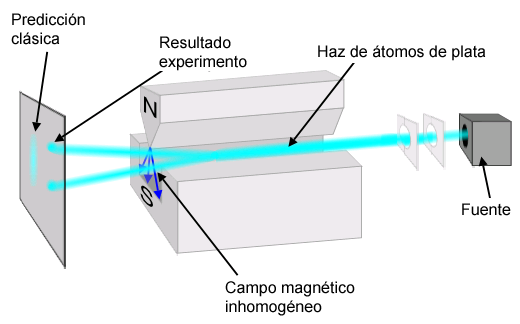
\includegraphics[scale=0.6]{Imagenes/Experimento_Stern-Gerlach_01.png}
    \caption{Créditos: CC BY-SA 3.0, \url{https://commons.wikimedia.org/w/index.php?curid=140004}}
\end{figure}
\end{frame}
\begin{frame}
\frametitle{Valores cuantizados del espín}
\begin{figure}
    \centering
    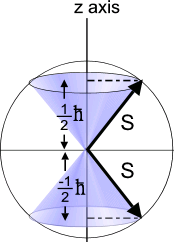
\includegraphics[scale=0.6]{Imagenes/Experimento_Stern-Gerlach_02.png}
    \caption{Créditos: De English Wikipedia user Theresa Knott, CC BY-SA 3.0., \url{https://commons.wikimedia.org/w/index.php?curid=5055540}}
\end{figure}
\end{frame}

\section{Condición de completitud.}
\frame{\tableofcontents[currentsection, hideothersubsections]}
\subsection{Los kets como conjunto completo}

\begin{frame}
\frametitle{Eigenkets como conjunto completo}
Acabamos de afirmar que los eigenkets de un observable forman un conjunto completo.
\\
\bigskip
\pause
Sea $\ket{n}, n = 0, 1, 2, \ldots$ denota estos eigenkets y sea $\ket{P}$ que denota un ket arbitrario.
\end{frame}
\begin{frame}
\frametitle{Estados continuos}
Por lo tanto:
\pause
\begin{align*}
\ket{P} = \nsum_{n} c_{n} \, \ket{n}
\end{align*}
donde la suma $\displaystyle \nsum$ denota una suma sobre los estados discretos y una integración sobre los estados continuos.
\end{frame}
\begin{frame}
\frametitle{Eigenkets como conjunto ortonormal}
Dado que se puede suponer que los eigenkets forman un conjunto ortonormal $(\ip{m}{n} = \delta_{mn})$ tenemos:
\pause
\begin{align*}
\braket{m}{P} = \nsum_{n} c_{n} \braket{m}{n} = \nsum_{n} c_{n} \, \delta_{mn} = c_{m}
\end{align*}
\end{frame}
\begin{frame}
\frametitle{Resultado consecuente}
Por lo tanto:
\pause
\begin{align*}
\ket{P} = \nsum_{n} \ket{n} \, c_{n} = \left\{ \nsum_{n} \dyad{n} \right\} \, \ket{P}
\end{align*}
\end{frame}
\begin{frame}
\frametitle{Conclusión importante}
Dado que la ecuación anterior es válida para un ket arbitrario $\ket{P}$, la cantidad dentro de las llaves deben ser un operador de unidad:
\pause
\begin{align*}
\nsum_{n} \dyad{n} = 1
\end{align*}
que generalmente se conoce como \emph{condición de completitud}.
\end{frame}
\end{document}